%%%%%%%%%%%%%%%%%%%%%%%%%%%%%%%%%%%%%%%%%
% a0poster Landscape Poster
% LaTeX Template
% Version 1.0 (22/06/13)
%
% The a0poster class was created by:
% Gerlinde Kettl and Matthias Weiser (tex@kettl.de)
% 
% This template has been downloaded from:
% http://www.LaTeXTemplates.com
%
% License:
% CC BY-NC-SA 3.0 (http://creativecommons.org/licenses/by-nc-sa/3.0/)
%
%%%%%%%%%%%%%%%%%%%%%%%%%%%%%%%%%%%%%%%%%

%----------------------------------------------------------------------------------------
%	PACKAGES AND OTHER DOCUMENT CONFIGURATIONS
%----------------------------------------------------------------------------------------

\documentclass[a0,landscape]{a0poster}

\usepackage{multicol} % This is so we can have multiple columns of text side-by-side
\columnsep=100pt % This is the amount of white space between the columns in the poster
\columnseprule=3pt % This is the thickness of the black line between the columns in the poster

\usepackage[svgnames]{xcolor} % Specify colors by their 'svgnames', for a full list of all colors available see here: http://www.latextemplates.com/svgnames-colors

\usepackage{times} % Use the times font
%\usepackage{palatino} % Uncomment to use the Palatino font

\usepackage{graphicx} % Required for including images
\graphicspath{{figures/}} % Location of the graphics files
\usepackage{booktabs} % Top and bottom rules for table
\usepackage[font=small,labelfont=bf]{caption} % Required for specifying captions to tables and figures
\usepackage{amsfonts, amsmath, amsthm, amssymb} % For math fonts, symbols and environments
\usepackage{wrapfig} % Allows wrapping text around tables and figures

\usepackage{caption}
\usepackage{subcaption}

\begin{document}

%----------------------------------------------------------------------------------------
%	POSTER HEADER 
%----------------------------------------------------------------------------------------

% The header is divided into three boxes:
% The first is 55% wide and houses the title, subtitle, names and university/organization
% The second is 25% wide and houses contact information
% The third is 19% wide and houses a logo for your university/organization or a photo of you
% The widths of these boxes can be easily edited to accommodate your content as you see fit

\begin{minipage}[b]{0.55\linewidth}
\veryHuge \color{NavyBlue} \textbf{Recidivism of Criminal Offenders} \color{Black}\\ % Title
\Huge\textit{A machine-learning approach to justice}\\[1cm] % Subtitle
\huge \textbf{Estienne Granet \hspace{8.7cm}    Victor Lei}\\ % Author(s)
\Large \texttt{egranet@g.harvard.edu} \hspace{6cm} \texttt{vlei@g.harvard.edu}\\ % Author(s)
\Large Harvard University \hspace{12.3cm} Harvard University\\ % University/organization
\end{minipage}


\vspace{1cm} % A bit of extra whitespace between the header and poster content

%----------------------------------------------------------------------------------------

\begin{multicols}{4} % This is how many columns your poster will be broken into, a poster with many figures may benefit from less columns whereas a text-heavy poster benefits from more

%----------------------------------------------------------------------------------------
%	ABSTRACT
%----------------------------------------------------------------------------------------

\color{Navy} % Navy color for the abstract

\begin{abstract}

Recidivism of criminal offenders is a difficult topic in criminal justice. If we view the justice system as serving an important rehabilitatory purpose, then recidivism represents indicators for potential improvement in the correctional system. Using a public data-set on two cohorts of inmates released from North Carolina prisons in 1978 and 1980, we build two predictors of whether an individual will offend again in the future. Our first predictor is one-layer feed-forward neural networks. The second predictor is random forest. Results are presented below.

\end{abstract}

%----------------------------------------------------------------------------------------
%	INTRODUCTION
%----------------------------------------------------------------------------------------

\color{SaddleBrown} % SaddleBrown color for the introduction

\section*{Introduction}

Our goal is to effectively forecast whether an offender will offender again in the future when he or she is released from prison. To achieve this goal, we rely on a survey conducted on prisoners released from North Carolina prisons in 1978 and 1980. The survey contains questions on the background of the offenders, including their involvement in drugs or alcohol, level of schooling, nature of the crime resulting in the sample conviction, number of prior incarcerations and recidivism following release from the sample
incarceration. The data collection also contains information on the
the marital status, the sex, the age and the race of the offenders. In hard numbers, the dataset contains 9,327 profiles for prisoners released in 1978 and 9,549 profiles for prisoners released in 1980. Each entry has 16 variables and most variables are indicators.

\paragraph{}
Past work on the topic include an article on recidivism prediction \cite{bib1}. In the article, Palocsay et al. fit a one-layer neural network model on the data set, thus providing us with a reference for comparison. Historically though, recidivism prediction has been based on explicative models borrowed from survival analysis such as \cite{bib2} or \cite{bib3}.


\color{DarkSlateGray} % DarkSlateGray color for the rest of the content

\section*{Neural Network}
Neural networks were discovered some time ago, but lately, they have been experiencing a resurgence in usage. There is likely significant complexity in the interactions between the different variables, so simple models like logistic regression are not going to be as capable of modeling them compared to neural networks. Prior work on this data set has considered the use of neural networks and found them to have good predictive power for recidivism compared to traditional modeling techniques like logistic regression models. We seek to harness the improvements in neural networks that have been made over the last few years in an attempt to improve predictive accuracy. We find that we can achieve a small, but notable improvement in accuracy on unseen data.

As this is a plain binary classifications problem, we use a multi-layer perceptron feedforward neural network with a single hidden layer, bias terms, and the logistic function as the activation function ($f$) for both the hidden and output layers. There is a single output neuron ($\hat{y} \in (0, 1)$) used for classification with a $0.5$ threshold. For some input vector $x$, linear weights $W$, and bias terms $b$:

\[ \hat{y} = f( W_2  f( W_1 x + b_1 ) + b_2 ) \]
\[ E = - y \ln( \hat{y} ) - (1 - y) \ln ( 1 - \hat{y} ) \]

\begin{center}\vspace{1cm}
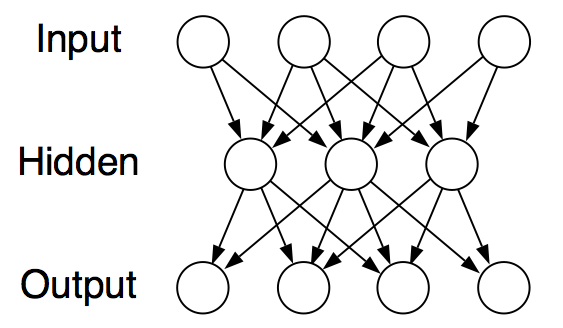
\includegraphics[width=0.8\linewidth]{neural_network}
\captionof{figure}{\color{Green} Feedforward Neural Network\cite{jordan2004introduction}}
\end{center}\vspace{1cm}

Using cross-entropy error ($E$), we can apply backpropagation and optimize the weights and bias terms by stochastic gradient descent using $\frac{\partial E}{\partial W}$, and $\frac{\partial E}{\partial b}$. In order to counteract overfitting, we use an early-stopping heuristic to stop training the model when the validation set performance does not improve for a certain number of epochs.

\begin{wraptable}{l}{12cm} % Left or right alignment is specified in the first bracket, the width of the table is in the second
\begin{tabular}{l l l}
\toprule
\textbf{Dataset} & \textbf{Palocsay et al.} & \textbf{Our results}\\
\midrule
1978 & 69.20\% (39) & 70.69\% (9) \\
1980 & 66.98\% (26) & 68.22\% (5) \\
\bottomrule
\end{tabular}
\captionof{table}{\color{Green} Validation set performance for NN predictor}
\end{wraptable}

After splitting the 1978 dataset and the 1980 dataset into training and validation sets (7:3 ratio) and training the neural network, validation set performance is improved compared to the results from Palocsay et al \cite{bib1}. The results are also achieved with far fewer nodes in the hidden layer, making it faster to train and likely more generalizable. As the figures below reveal, the neural network starts to quickly overfit as the number of nodes in the hidden layer increases.

\begin{center}\vspace{1cm}
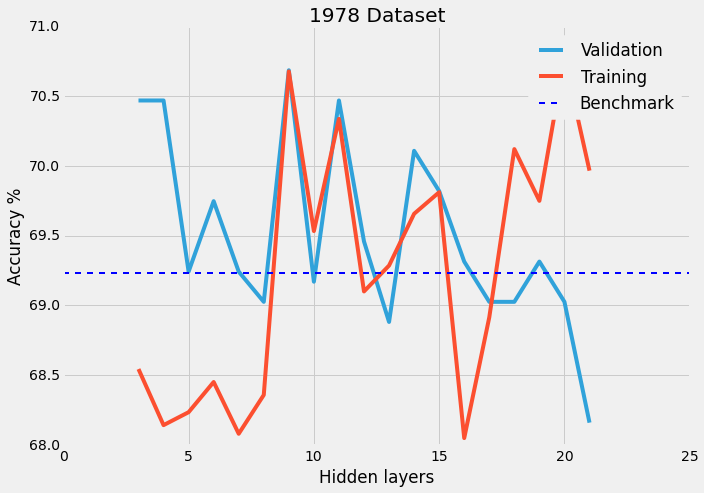
\includegraphics[width=0.9\linewidth]{1978}
\captionof{figure}{\color{Green} 1978 Dataset}
\end{center}\vspace{1cm}

%\begin{center}\vspace{1cm}
%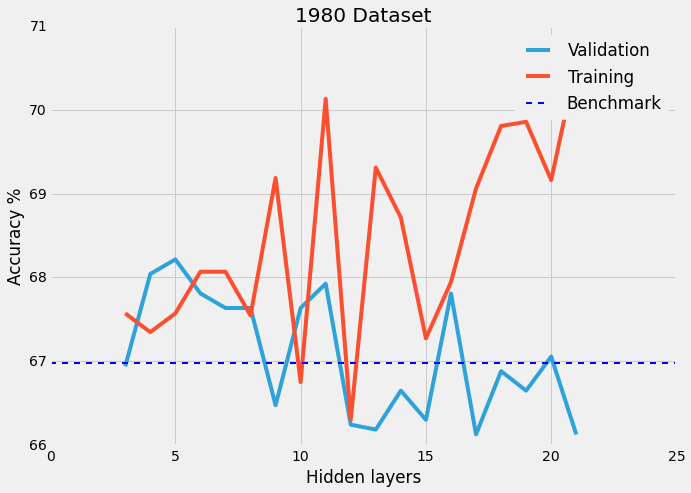
\includegraphics[width=0.9\linewidth]{1980}
%\captionof{figure}{\color{Green} 1980 Dataset}
%\end{center}\vspace{1cm}

\section*{Random Forest}

A Random Forest predictor was built over the data in order to get some sense of what features were significantly impacting the odds of recidivism. Two loss functions - a Gini loss and an entropy loss - were tested without any conclusion difference. We simulated over a number of trees ranging from $10$ to $100$, as higher values were not bringing any noticeable improvement. The number of features tested ranged from $1$ to all. The figure below gives an idea of the best features.

\begin{center}\vspace{1cm}
  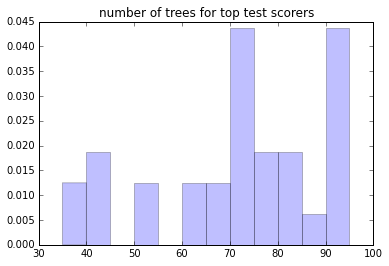
\includegraphics[width=.45\linewidth]{number_forest78.png}
  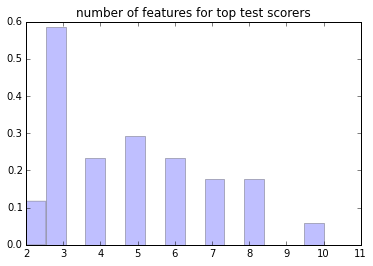
\includegraphics[width=.45\linewidth]{number_features78.png}
\captionof{figure}{\color{Green} Number of trees and number of features for the top 5\% test scores.  Simulations were performed for a feature number ranging from $1$ to all, a number of trees ranging from $10$ to $100$, and a Gini loss.}
\end{center}\vspace{1cm}

\paragraph{}
The best result were obtained for a test set reduced to 10\% of the initial dataset - in this case, the top test score repeatedly reach 71 \% as we shuffle over and over test and training sets. When we use the NN splitting ratio (7 : 3), we obtain the following results.

\begin{center}\vspace{1cm}
\begin{tabular}{l l l}
\toprule
\textbf{Dataset} & \textbf{Score on test set} \\
\midrule
1978 & 67.46 \%  \\
1980 & 67.95 \%  \\
\bottomrule
\end{tabular}
\captionof{table}{\color{Green} Best performance for the Random Forest predictor. Test set is identical for NN and Random Forest.}
\end{center}\vspace{1cm}


\section*{Remarks on the dataset}

\paragraph{Score plateau}
The score on the test set seems to have an upper bound at $72$\%, independently of the classification method. One explanation of this plateau is the existence of antagonist duplicates in the data set, that is to say two individuals with very similar features but one is a recidivist and the other is not. Such duplicates would structurally lower the score. The existence of duplicates is made easier by the fact that $13$ of the $16$ feature variable are indicator functions. To address the concern, we looked at the data set. All non-indicator variables were partitioned in groups. For example, the age variable (expressed in months) was replaced with a categorical variable that indicates whether the individual belongs to age group $[0,19], [20, 24], [25,29], [30,34], \dots$. Depending on how we define these groups, we get a duplicate rate between $1$ \% and $10$ \%, which is only a partial explanation for the plateau. Another is simply the lack of data. The $11$ indicator variables represent $2^11 = 2048$ combinations. If we add $5$ non-indicator categorical variables, we get a a number of combinations that is significantly bigger than $9,327$, the number of data points for prisoners released in 1978 or even the total number of data points if we merge the $1978$ and $1980$ files.

\paragraph{Explicative variables}
Random forests classifiers indicate that the number of years spent at school, the age and the duration of the sentence were more important features. This result should be treated cautiously as these three variables happen to be the only 3 variables that are not indicators. Their discriminative power is consequently strengthened.

\begin{center}\vspace{1cm}
  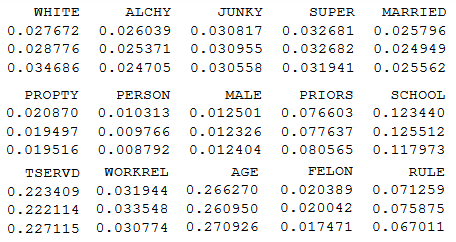
\includegraphics[width=\linewidth]{features_weights.png}
\captionof{figure}{\color{Green} Importance weights for  the top 2 test scores among all classifiers simulated.}
\end{center}\vspace{1cm}


%----------------------------------------------------------------------------------------
%	CONCLUSIONS
%----------------------------------------------------------------------------------------

\color{SaddleBrown} % SaddleBrown color for the conclusions to make them stand out

\section*{Conclusions}

We improve upon the existing work done by Palocsay et al. \cite{bib1} on this data set by achieving a higher validation set accuracy using fewer nodes in the hidden layer. The random forest classifiers indicated that the main factors involved in recidivism are the age, the time served in jail and the level of education.


\color{DarkSlateGray} % Set the color back to DarkSlateGray for the rest of the content

%----------------------------------------------------------------------------------------
%	FORTHCOMING RESEARCH
%----------------------------------------------------------------------------------------

\section*{Forthcoming Research}

We are still exploring other ways of optimizing the neural network and more advanced regularization strategies like Dropout. In parallel, we are looking into a hierarchical mixture of models (HME). We hope that a HME will be less prone to local maxima - a frequent problem in our simulations.

 %----------------------------------------------------------------------------------------
%	REFERENCES
%----------------------------------------------------------------------------------------

\nocite{*}
\bibliographystyle{unsrtnat}
\bibliography{sample}


\end{multicols}
\end{document}